\documentclass[12pt, oneside]{article}
\usepackage[T1]{fontenc}
\usepackage[spanish, es-tabla, es-lcroman]{babel}
\usepackage[utf8]{inputenc}
\usepackage[document]{ragged2e}
\usepackage{tcolorbox}
\tcbuselibrary{theorems}
\usepackage{cancel}
\usepackage{amssymb}
\usepackage{amsmath}
\usepackage{mathrsfs}
\usepackage{wrapfig}
\usepackage{fancyhdr}
\usepackage{colortbl}
\usepackage{diagbox}
\usepackage{longtable}
\usepackage{graphicx}
\usepackage{subcaption}
\usepackage{xcolor}
\usepackage{tikz}
\usetikzlibrary{positioning}
\usepackage{multicol}
\usepackage{multirow}
\usepackage{lastpage}
\usepackage{pdfpages}
\usepackage{listings}
\usepackage{blindtext}
\spanishdecimal{.}
\usepackage[explicit]{titlesec}
\usepackage[colorlinks=true, linkcolor=black, citecolor=black, urlcolor=blue]{hyperref}
\usepackage[a4paper, total={16cm, 24cm}]{geometry}
\pagestyle{fancy}
\lhead{Muñoz Nuñez Ian Emmanuel}
\rhead{Practica 12}
\lfoot{Mtra. María Patricia Ventura Nuñez}
\rfoot{CUCEI}
\renewcommand{\headrulewidth}{1pt}
\renewcommand{\footrulewidth}{1pt}

\setlength{\headheight}{14.49998pt}

\begin{document}

\begin{titlepage}
    \pagenumbering{roman}
    \centering
    {\bfseries\LARGE Universidad de Guadalajara \par}
    \vfill
    {
        \includegraphics[width=0.3\linewidth]{UdG.png}
        \includegraphics[width=0.3\linewidth]{qci.png}
        \par
    }
    \vfill
    {\bfseries\LARGE Seminario de programación de sistemas reconfigurables \par}
    \vfill
    {\ttfamily\LARGE Animación con matriz de led's \par}
    \vfill
    {\bfseries\LARGE Nombre: \par}
    \vfill
    {\bfseries\LARGE Muñoz Nuñez Ian Emmanuel \par}
    \vfill
    {\bfseries\LARGE Sección: D01 \par}
    \vfill
    {\bfseries\LARGE Código: 216464457 \par}
    \vfill
    {\bfseries\LARGE Maestra: \par}
    \vfill
    {\bfseries\LARGE María Patricia Ventura Nuñez \par}
    \vfill
    {\bfseries\LARGE Ingeniería Robótica \par}
\end{titlepage}

\pagenumbering{arabic}

\newpage
\section{Objetivo}
{\sffamily\large
    \hspace{0.5cm} Solucionar problemas de diseño utilizando las herramientas aprendidas en
    programación de sistemas reconfigurables.

    \hspace{0.5cm} Simular circuitos digitales en programas de diseño como
    \emph{Proteus\textregistered} e implementarlos físicamente.

    \hspace{0.5cm} Diseño codificación, simulación e implementación de figuras y letras que se
    desplacen a través de la matriz de led's.

}

\section{Material}
{\sffamily\large
    \renewcommand{\labelitemi}{$\bullet$}
    \begin{itemize}
        \item Protoboard.
        \item Fuente VCC (5V).
        \item Resistencias de $2.2k\Omega$.
        \item 3 contadores \emph{4029}.
        \item 1 demultiplexor \emph{74LS138}.
        \item 1 memoria ROM \emph{AT28C64B}.
    \end{itemize}

}

\section{Marco teórico}
{\sffamily\large
    \hspace{0.5cm} Para este proyecto lo complicado fue escribir el código hexadecimal para la
    memoria ROM \emph{AT28C64B}, pues, aunque se utilizo el software \emph{CodeGraphics}, fue algo
    tardado, otro problema encontrado en este proyecto fue pasar las conexiones de la matriz, pues
    en el software de simulación \emph{Proteus\textregistered} la matriz se muestra de una forma,
    pero el circuito físico de la matriz de led's es muy diferente al de la simulación, por
    último, el mayor problema fue cargar el programa en la memoria \emph{ROM}, pues por alguna
    razón, el programa no podia cargar el archivo hexadecimal a la memoria \emph{ROM}. Por esta
    razón, no se pudo probar el circuito en la protoboard.

}

\newpage
\subsection{Figuras utilizadas para el proyecto}
\begin{figure}[h!]
    \centering

    \begin{subfigure}{0.45\textwidth}
        \centering
        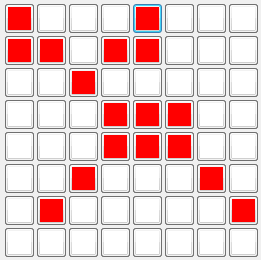
\includegraphics[width=\linewidth]{figs/reno.PNG}
    \end{subfigure}
    \begin{subfigure}{0.45\textwidth}
        \centering
        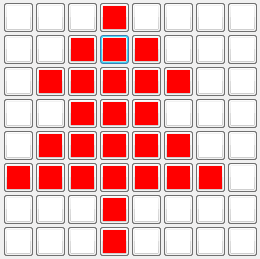
\includegraphics[width=\linewidth]{figs/pino.PNG}
    \end{subfigure}
    \begin{subfigure}{0.45\linewidth}
        \centering
        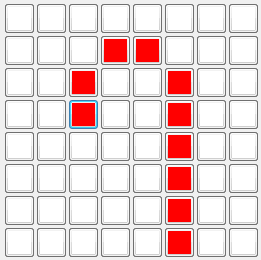
\includegraphics[width=\linewidth]{figs/baston.PNG}
    \end{subfigure}
    \begin{subfigure}{0.45\textwidth}
        \centering
        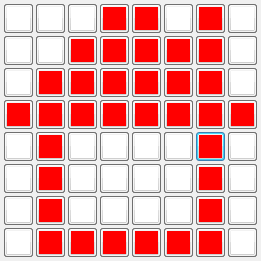
\includegraphics[width=\linewidth]{figs/casa.PNG}
    \end{subfigure}
    \begin{subfigure}{0.45\linewidth}
        \centering
        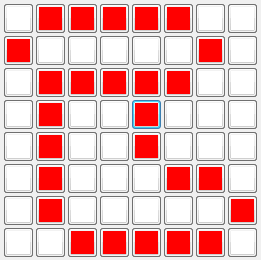
\includegraphics[width=\linewidth]{figs/bota.PNG}
    \end{subfigure}

    \caption{\sffamily Figuras utilizadas para el proyecto}
    \label{fig:figuras}
\end{figure}

\newpage
\section{Procedimiento}
{\sffamily\large
    \hspace{0.5cm} Para llevar a cabo este proyecto, primero se pensó en las figuras que se
    mostrarían en la matriz de led's, después, con ayuda del software \emph{CodeGraphics} se
    conseguia el código hexadecimal necesario para escribir el código hexadecimal que se cargaría
    a la memoria \emph{ROM}, conforme se creaba la animación se pasaba el código al programa
    \emph{Max Loader}, cada código se escribio 10 veces en la \emph{ROM} para que la memoria lo
    mostrara varias veces, y no pasara rápidamente. Luego de eso, solo se observó como se quería
    usar la matriz y como se quería la orientación de la matriz, y hacer las conexiones necesarias
    no fue complicado, pues solo se necesitaban los contadores \emph{4029} con una secuencia del 0
    al 15 y colocarlos en cascada para que cuando un contador se desbordara, otro pasara al
    proximo estado. De esa forma se accedia a una dirección de memoria distinta, mientras la
    memoria va cambiando poco a poco los valores de su salida, el demultiplexor va prendiendo y
    apagando cada uno de los ánodos rápidamente para poder mostrar la secuencia.

    \hspace{0.5cm} Los materiales utilizados para este circuito son: 8 resistencias de
    $2.2k\Omega$, 3 contadores \emph{4029}, 1 demultiplexor \emph{74LS138}, 1 matriz de led's
    de 8x8 y 1 memoria ROM \emph{AT28C64B}.

}

\section{Circuito a implementar}
\subsection{Simulación}
{\sffamily\large
    \hspace{0.5cm} En la siguiente página se muestra el diseño del circuito en simulación con el
    software \emph{Proteus\textregistered}.

    \newpage
    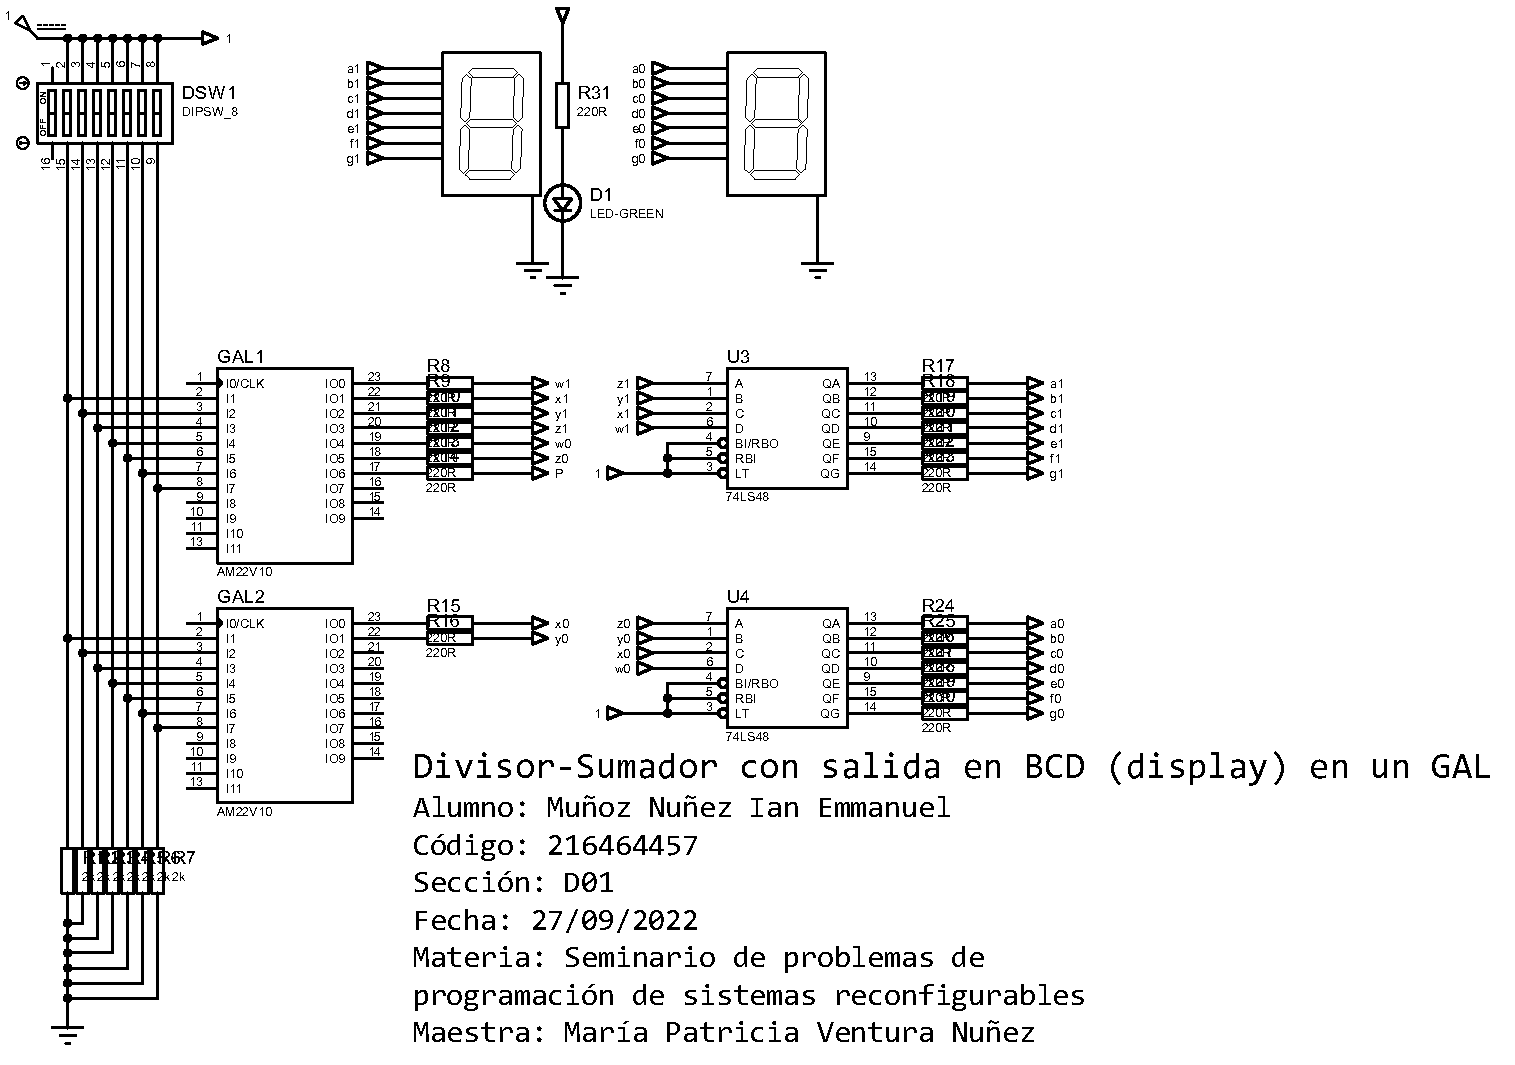
\includepdf[pages={1}]{main.PDF}

}

\subsection{Protoboard}
\begin{figure}[h!]
    \centering
    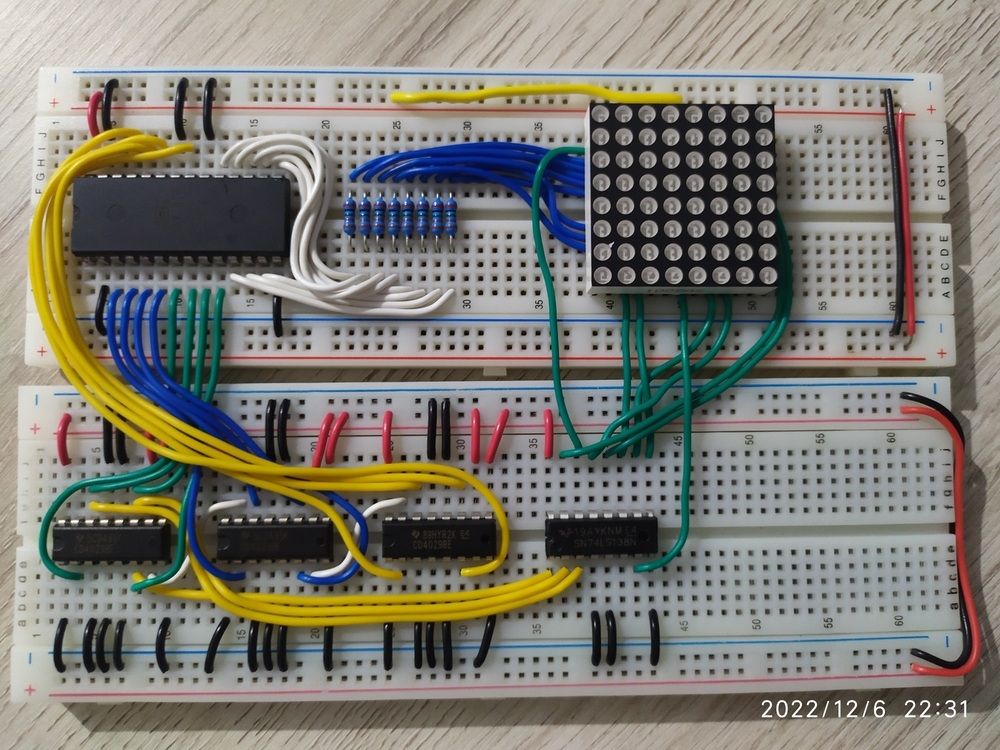
\includegraphics[width=0.8\linewidth]{figs/IMG_20221206_223112.jpg}
    \caption{\sffamily Circuito en protoboard}
    \label{fig:proto}
\end{figure}

\section{Conclusión}
{\sffamily\large
    \hspace{0.5cm} Este fue un circuito muy interesante y aunque fue muy complicado, en serio fue
    muy divertido hacerlo, aunque solo se pudo llevar a cabo en simulación, fue muy interesante
    entender aún más el funcionamiento de una memoria \emph{ROM} y entender como es que accede a
    cada una de sus localidades y/o direcciones, en serio me hubiera gustado mucho poder ver este
    circuito funcionando en físico, espero poder terminarlo y ver su funcionamiento.

}

\end{document}

